\chapter{Week 7: 2\textsuperscript{nd} - 8\textsuperscript{th} March }

\begin{itemize*}
	\item Acquire  data for \gls{gps} filter design
	\item  Find the \gls{noisecomatrix} for the \gls{gps} Kalman Filter.
	\item Test the Control on the Quad-rotor
	
\end{itemize*}

 \tocless\section{\gls{gps} data}
The following data was acquired during the course of the 

						\begin{figure}[h!]
							\centering
							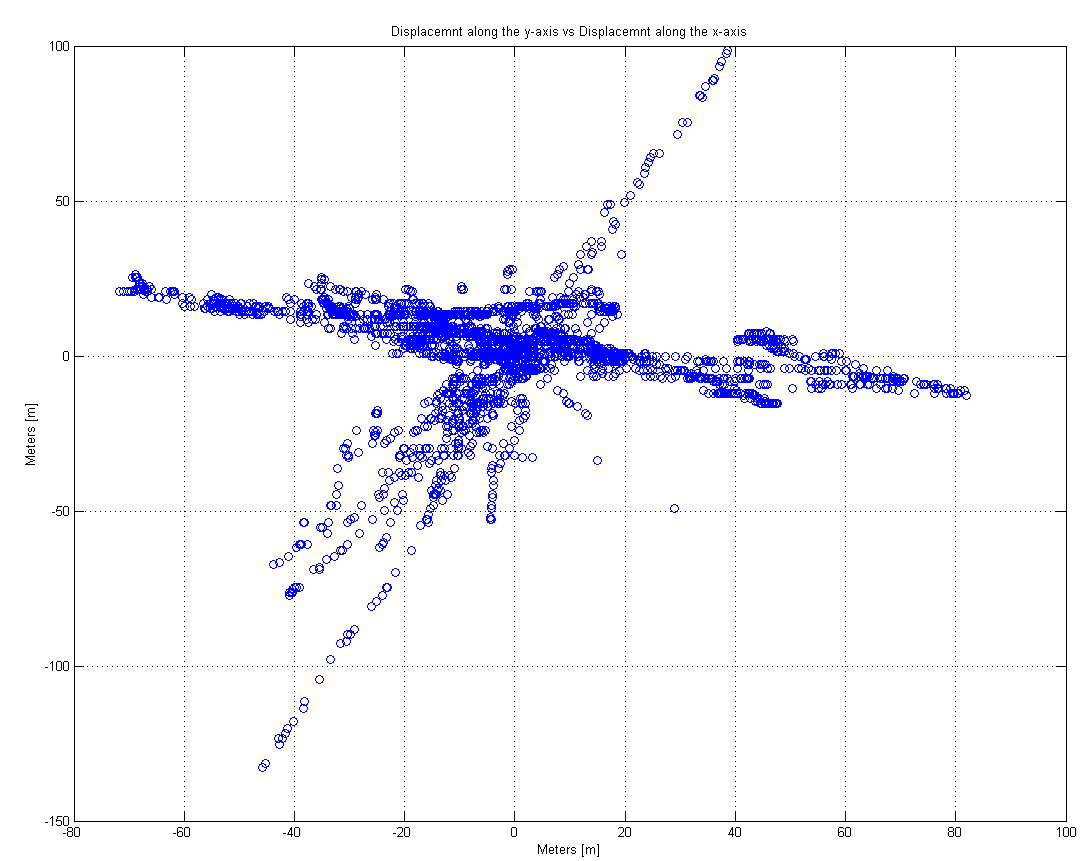
\includegraphics[width =0.7\paperwidth, height = 10cm]{\DocRoot/images/xy_plot_gps}
							\caption{Plot of \gls{gps} data in x-y plane}
							\label{Fig: Plot of gps data in x-y plane}
						\end{figure}

						\begin{figure}[h!]
							\centering
							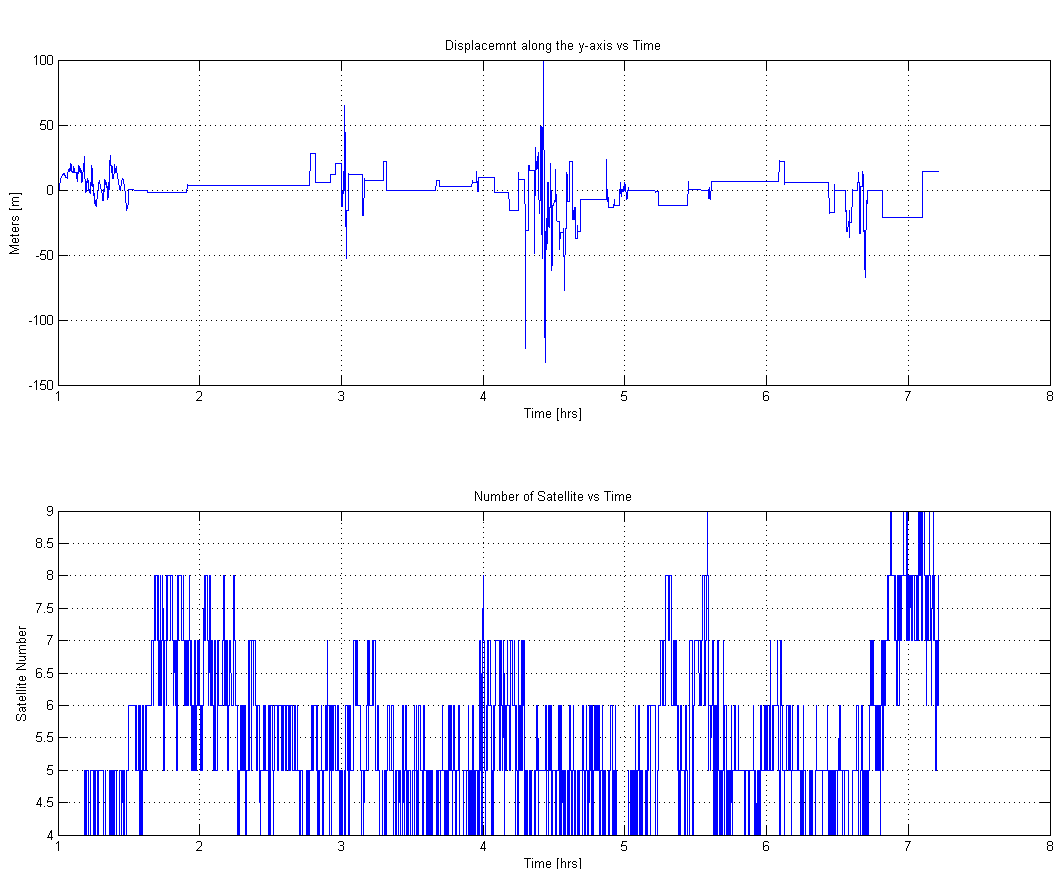
\includegraphics[width =0.5\paperwidth]{\DocRoot/images/x_plot_gps}
							\caption{Plot of \gls{gps} data in displacement in x direction vs time}
							\label{Fig: Plot of gps data in displacement in x direction vs time}
						\end{figure}

						\begin{figure}[h!]
							\centering
							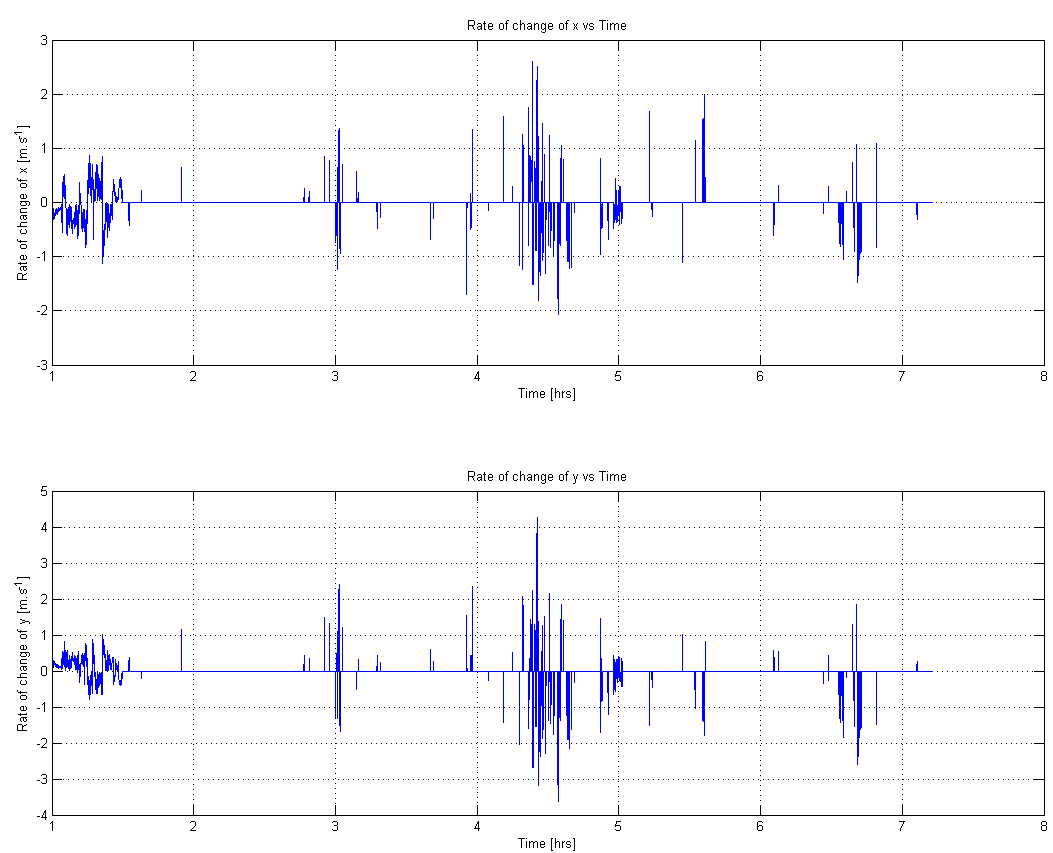
\includegraphics[width =0.5\paperwidth]{\DocRoot/images/x_rate_vs_time}
							\caption{Plot of \gls{gps} data in x rate vs time}
							\label{Fig: Plot of gps data in x rate vs time}
						\end{figure}


\newpage
 \tocless\section{Find the \gls{noisecomatrix} for the \gls{gps} Kalman Filter.}
From data collected the following \gls{noisecomatrix} where found for $x$ and $y$ respectively.
					\begin{equation}
					\gls{noisecomatrix}_{\gls{east}} = 		
					\left[\begin{array}{cc}
					\mathrm{cov(\gls{east})}       &                 0                          \\ 
					0                                                          & cov( \dot{x}_n   )          
					\end{array} \right]
					=					
					\left[\begin{array}{cc}
				 132.58    &                 0                          \\ 
					0                                                          & 0.0301         
					\end{array} \right]
					\end{equation}
					
										\begin{equation}
										\gls{noisecomatrix}_{\gls{north}} = 		
										\left[\begin{array}{cc}
										\mathrm{cov(\gls{north})}       &                 0                          \\ 
										0                                                          & cov( \dot{y}_n   )          
										\end{array} \right]
										=					
										\left[\begin{array}{cc}
										159.4762    &                 0                          \\ 
										0                                                          & 0.0617         
										\end{array} \right]
										\end{equation}
										
	 \tocless\section{\gls{gps} model used for Kalman Filter}			
	
	The $x$ model used by the kalman filter is defined as follows:-
						\begin{equation}
					\left[\begin{array}{c}
					\dot{\gls{east}}                          \\ 
					\ddot{\gls{east}}                                                          
					\end{array} \right] = 		
						\left[\begin{array}{cc}
					0       &                 1                         \\ 
						0                                                          &-\frac{ \gls{dampingx} }{\gls{systemmass}}        
						\end{array} \right]
				+
											\left[\begin{array}{c}
									      	0                         \\ 
											\frac{ 1 }{\gls{systemmass}}                                                       
											\end{array} \right] U					
						\end{equation}
and the $y$ modelled as follows.						
						\begin{equation}
						\left[\begin{array}{c}
						\dot{\gls{north}}                          \\ 
						\ddot{\gls{north}}                                                          
						\end{array} \right] = 		
						\left[\begin{array}{cc}
						0       &                 1                         \\ 
						0                                                          &-\frac{ \gls{dampingy} }{\gls{systemmass}}        
						\end{array} \right]
						+
						\left[\begin{array}{c}
						0                         \\ 
						\frac{ 1 }{\gls{systemmass}}                                                       
						\end{array} \right] U					
						\end{equation}
	
 \tocless\section{Test Quad-rotor}
Fixing issues with program run-time on Propeller and the quad-rotor was stabilised about the pitch and roll axis.						